\newpage
\subsection{CUDA}

The CUDA architechure was released for the first time in 2006 to make it easier to perform general purpose GPU-computing. Unlike previous methods that had to get around the old pipeline with vertex and fragment shaders, CUDA allowed every aritmethic logic unit on the chip to be controlled by a CUDA program. Another important feature was the possibility to read and write to arbitrary memory address on the GPU in comparison to previous methods that required textures as storage. The hardware was still in charge of memory caching but CUDA also exposed a software managed cache called shared memory. CUDA programs are written in the CUDA C language, a language very close to the C language with the exception of a small number of keywords added for special features in the CUDA architecture.  

\subsubsection{Blocks and threads}

In the CUDA architechure, threads are single execution units that run kernels on the GPU. They are similar to CPU threads but the typically there are a lot more of them on the GPU. The threads are divided into thread blocks. Threads within a thread block can communicate with each others. The number of blocks and threads per block is decided by the developer when the kernel is called. The grid of block can be one, two or three dimensional. The maximum number of blocks and threads per block is decided by the GPU and its hardware. A CUDA kernel is executed simulatenously by warps. A warp consists of threads within a block. Typically each warp has the size of 32 threads, where actions like memory read and writes are performed in half-warps. 
\newline

\begin{figure}[ht!]
\centering
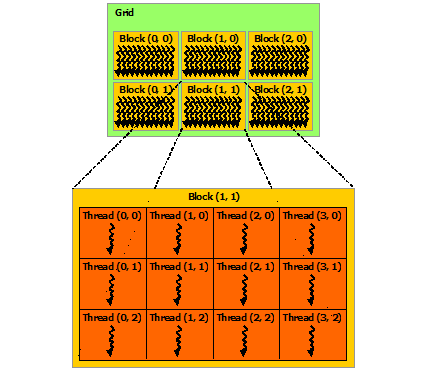
\includegraphics[width=80mm]{img/grid-of-thread-blocks.png}
\caption{CUDA threads divided into blocks of threads.}
\label{cudablockthreads}
\end{figure}

\renewcommand{\lstlistingname}{Code}
\begin{lstlisting}[caption= Example of vector addition in CUDA, label=cuda1]
__global__ void VectorAddition(float * A, 
                               float * B, 
                               float * C)
{
    int i = blockIdx.x * blockDim.x + threadIdx.x;
    int j = blockIdx.y * blockDim.y + threadIdx.y;
    int idx = i + j * gridDim.x * blockDim.x;
    C[idx] = A[idx] + B[idx];
}
\end{lstlisting}

When a thread is executing a kernel, there are built-in variables to access information of which block the thread belongs to and the local thread index in the actual block. This is often used to know where to read and write in a global array. Code \ref{cuda1} shows an example of a simple CUDA kernel performing a vector addition. The keyword \texttt{\_\_global\_\_} is used to tell the compiler that the function is a CUDA kernel. The variables \texttt{blockIdx}, \texttt{threadIdx}, \texttt{gridDim} and \texttt{blockDim} are automatically built-in in a CUDA kernel and can be accessed at any time. \texttt{blockIdx} and \texttt{threadIdx} are of the type \texttt{uint3}, where each value represent an index in the corresponding dimension. \texttt{blockIdx} is the index of the block in the total grid of launched blocks and \texttt{threadIdx} is the thread index within the block. Both \texttt{gridDim} and \texttt{blockDim} are of the type \texttt{dim3} and are constant in all threads (not possible to launch a kernel with different block sizes).

\subsubsection{Memory hierarchy}
\begin{figure}[ht!]
\centering
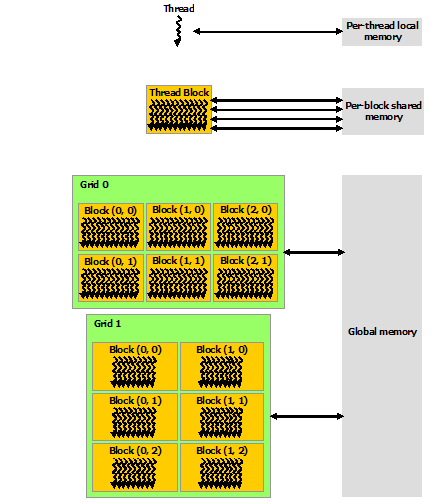
\includegraphics[]{img/memory-hierarchy.png}
\caption{Different CUDA memory spaces}
\label{cudamemoryhierarchy}
\end{figure}
There are differnet memory spaces in the CUDA architechure as can be seen in Figure \ref{cudamemoryhierarchy}. Each thread has a local and private memory space. All the threads in a block can share a memory space, called shared memory. Shared memory is on-chip and is divided into different banks. Reading from shared memory in warp of threads is just as fast as reading from a register as long as there are no bank conflicts. Each bank conflict results in a serialized read from the shared memory. Worst case scenario is when all threads in a warp only read from one bank in the shared memory. The shared memory read then becomes a lot slower then the regular global memory. Global, constant and texture memory can all all be accessed by all threads. Constant and texture memory are only used in certain cases where the global memory is the common choice for storing data. The texture memory space is cached to that a texture fetch only cost a GPU device memory read on a cache miss, otherwise it only costs a read from the texture cache. Texture cache is optimized for 2D spatial locality. If desired, one also gets an automatic linear interpolation when reading from the texture space. Constant memory is a read-only memory space. All the threads of a half-warp read from constant memory just as fast as from a register as long as all the threads read from the same address. The cost scales linearly with the number of different addressed read by the threads. For example, the worst case would be if an array would be stored in the constant memory space and each thread in an executing half-warp needs an unique value in this array. The commonly used global memory space is capable of reading 4, 8 and 16 bytes of memory into registers in one single instruction. The most efficient global memory reads are when all threads in a half-warp reads from continous memory in a coalesced read of 64, 128 or 256 bytes. It is impossible for a thread to know if the current value in the global memory  has been updated or not if a kernel is reading and writing to the same global memory. CUDA supports atomic operations but they are usually slow and a common technique is to have to different buffers allocated, one to read from and one to write to.



